\documentclass[12pt,a4paper,oneside,brazil]{abntex2}

% Pacotes que serão utilizados%
\usepackage{lmodern}
\usepackage[utf8]{inputenc}
\usepackage[brazil]{babel}
\usepackage[T1]{fontenc}
\usepackage{indentfirst}
\usepackage{graphicx}
\usepackage{microtype}
\usepackage{wrapfig}
\usepackage{amsmath}
\usepackage[backend = biber, style=abnt]{biblatex}
\addbibresource{Referencias.bib}

% Informações do documento %
\title{Notas Econometria I}
\author{Thiago Oliveira Coelho}
\date{\today}



\begin{document}
\pagestyle{plain}
\pagenumbering{arabic}

\maketitle\
\begin{center}
Resumo baseado em \cite{gujarati} e \cite{wooldridge}
\end{center}
\tableofcontents

\chapter{1ª Unidade}

\section{Análise de Regressão Simples}
É usada para determinar o impacto ceteris paribus entre variáveis. Seu modelo simples é o seguinte:
\[ Y = \beta_0 + \beta_1 X + u \]
Aonde:
\begin{itemize}
\item Y: Variável dependente;
\item X: Variável independente;
\item $\beta_0$: Intercepto (Valor de Y quando X = 0);
\item $\beta_1$: Coeficiente do impacto de X em Y;
\item u: Erro. Inclui todos os fatores que influenciam Y e não estão explicitados no modelo como variáveis explicativas.
\end{itemize}
Tanto X quanto u serão tratadas como variáveis aleatórias. Mas para capturar o efeito ceteris paribus das variáveis explicativas nós assumimos que $E(u) = 0$. Com isso podemos derivar também que : $E(u|x) = E(u) = 0$. Isso permite que X tenha um efeito \emph{linear} em Y. \newline
Encontramos assim nossa \emph{Função regressão populacional} [FRP]:
\[ E(Y|X) = \beta_0 + \beta_1 X\]

\begin{wrapfigure}{l}{0.5\textwidth}
	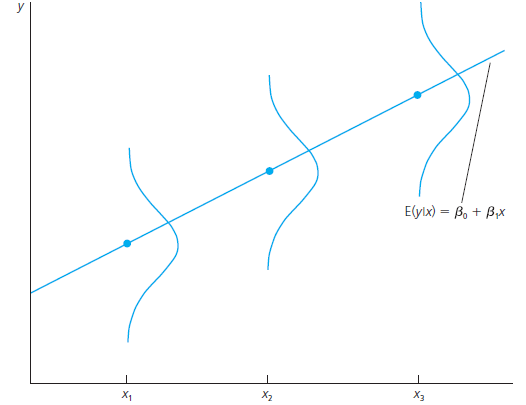
\includegraphics[width=0.5\textwidth]{OLS.png}
	\centering
	\caption{Fonte: \cite{wooldridge}}
\end{wrapfigure}

Observe que para cada observação de X há uma distribuição de valores de Y, mas os que estão na linha de regressão representam a esperança (média) destes valores para aquele dado X. A linha de regressão é o local geométricos das expectativas condicionais das variáveis dependentes dados certos valores das explicativas.
\clearpage
\section{Função Regressão Amostral [FRA]}
Dada uma amostra da população, existe uma reta de regressão que define esta amostra. Porém não é possível se obter esta reta pura por causa da pertubação estocástica (u). Portanto iramos achar estimativas dos parâmetros:
\[ \hat{Y} = \hat{\beta_0} + \hat{\beta_1} X_i \]
Aonde os betas não são seus valores reais, mas sim os \emph{estimadores} obtidos a partir da amostra, representados pelo chapéu.

\section{Estimativa de $\beta$ por mínimos quadrados ordinários}

\subsection{MQO / OLS}
Pelas hipóteses podemos deduzir:
\[ E(u) = Cov(x,u) = E(X u) = 0 \]
\[ u = Y - \beta_0 - \beta_1 X\]
\[E(X (Y - \beta_0 - \beta_1 X)) = 0 \]\\
Montamos o sistema:
\begin{equation} \label{beta0}
 \frac{\sum_{i=1}^{n} Y_i - \hat{\beta}_0 - \hat\beta_1 X_i}{n} = 0 
 \end{equation}
 \begin{equation} \label{beta1}
\frac{\sum_{i=1}^{n} X_i (Y_i - \hat{\beta}_0 - \hat{\beta}_1 X_i)}{n} = 0
 \end{equation}
Pelas regras de somatório:
\[ \frac{\sum_{i=1}^{n} Y_i}{n} -\frac{\sum_{i=1}^{n} \hat{\beta}_0}{n} - \frac{\sum_{i=1}^{n} \hat{\beta}_1 X_i}{n} = 0 \]
\[  \hat{\beta}_0 = \overline{Y} - \hat{\beta}_1 \overline{X} \]
Substituindo o valor de $\beta_0$ na segunda equação:
\[\sum_{i=1}^{n} X_i (Y_i - ( \overline{Y} - \hat{\beta}_1 \overline{X}) - \hat{\beta}_1 X_i = 0 \]
Por manipulação algébrica chegamos no seguinte sistema de equações linear (Todos os betas são estimativas):
\[ \hat{\beta}_0 = \overline{Y} - \hat{\beta}_1 \overline{X} \]
\[\hat{\beta}_1 = \frac{ \sum_{i=1}^{n} ( X_i - \overline{X}) ( Y_i - \overline{Y})}{{\sum_{i=1}^{n} ( X_i - \overline{X})^2}} \]
Percebe que a estimativa de beta 1 chapéu é dada pela covariância entre X e Y sobre a variância de X, portanto o sistema fica:
\begin{equation}\label{beta0chapeu}
 \hat{\beta}_0 = \overline{Y} - \hat{\beta}_1 \overline{X} 
\end{equation}
\begin{equation} \label{beta1chapeu}
\hat{\beta}_1 = \frac{Cov(X,Y)}{Var(X)} 
\end{equation}

\subsection{Soma dos quadrados dos resíduos}
O resíduo de uma observação é dada por:
\[ \hat{u}_{i} = Y_i - \hat{Y}_{i} = Y_i - (\hat{\beta}_0 + \hat{\beta}_1 X_1) \]
Existem n resíduos, que nos dizem a diferença entre os valores esperados de $Y$ estimados pelo modelo e os valores das observações.
\begin{figure}[h]
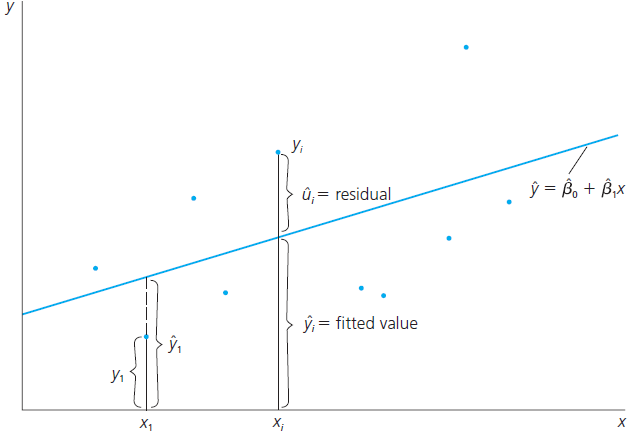
\includegraphics[scale=0.7]{Residual.png}
\centering
\caption{Fonte: \cite[p. 28]{wooldridge}}
\end{figure}
\[ \sum_{i = 1}^{n} \hat{u}_i^2 \]
A idéia é obter uma reta com o menor resíduo possivel, para isso queremos minimizar a soma dos quadrados dos resíduos:
\[ \sum_{i = 1}^{n} Y_i - \hat{Y}_i\]
Substituímos $Y_i$ e obtemos a equação final:
\[  Q= \sum_{i = 1}^{n} ( Y_i - \hat{\beta}_0 - \hat{\beta}_1 X_i)^2 \]
Com isso nosso objetivo passa a ser minimizar $Q$ com relação a $\hat{\beta}_0$ e $\hat{\beta}_1$.
\clearpage
Teremos então as condições de 1ª ordem:
\[\frac{dQ}{d \hat{\beta}_0} = 0 \rightarrow -2 \sum^n_{i=1} (Y_i - \hat{\beta}_0 - \hat{\beta}_1) \]
\[ \frac{dQ}{d \hat{\beta}_1} = 0 \rightarrow  -2 \sum^n_{i=1} X_i (Y_i - \hat{\beta}_0 - \hat{\beta}_1)\]
Podemos ainda fazer uma transformação monotônica das duas equações dividindo ambas por $-2$ e obter:
 \[\sum_{i = 1}^{n} ( Y_i - \hat{\beta}_0 - \hat{\beta}_1 X_i) \]
 \[\sum_{i = 1}^{n} X_i ( Y_i - \hat{\beta}_0 - \hat{\beta}_1 X_i) \]
 Que equivale ainda as duas hipóteses populacionais a quais chegamos ao tentar deduzir as fórmulas dos estimadores \ref{beta0} e \ref{beta1}. Se continuarmos a desenvolver as fórmulas chegariamos ao mesmo sistema para determinarmos os estimadores: \ref{beta0chapeu} e \ref{beta1chapeu}. Concluimos então que as fórmulas do estimadores minimizam a soma dos quadrados dos resíduos. \newline
 
 \section{Reta de regressão}
 A reta de regressão é aquela que minimiza os resíduos quadrados, que, como vimos anteriormentes, é aquela reta que tem como intercepto $\hat{\beta_0}$ e como inclinação $\hat{\beta_1}$. A reta de regressão passa por todos os valores esperados dado x e consegue te dar os valores previstos $\hat{Y}$ para todo valor de variável explicativa, até mesmo aquelas que não possuimos observações.
 \[ \frac{d\hat{Y}}{dx} = \hat{\beta_1} \Rightarrow \triangle \hat{Y} = \hat{\beta_1} \triangle X \]
A mudança em $ \hat{Y}$ é igual a mudança em $X$ vezes o coeficiente da reta $\hat{\beta_1}$. Esta previsão vale para a população como um todo.

\section{Forma funcional}
Um modelo é linear por causa de seus parâmetros, não por suas variáveis explicativas ou variável dependente. Todos os modelos a seguir são lineares, consequentemente nós podemos utilizar mínimos quadrados para obtermos seus coeficientes:
\[ \log Y = \beta_0 + \beta_1 X^2+ u \]
\[ Y = \beta_0 + \beta_1 \frac{1}{X} + u \]

Temos quatro principais formas funcionais:
\begin{enumerate}
\item Linear em Y e X $\rightarrow Y = \beta_0 + \beta_1 X + u$, neste caso $\frac{d Y}{d X} = \beta_1$.
\item Log em Y e  X $ \rightarrow \log Y = \beta_0 + \beta_1 \log X + u$, neste caso $\frac{d \log Y}{d \log X} = \beta_1 \approx \epsilon_{yx}$. $\beta_1$ indica a mudança percentual em Y dada alteração de 1\% em X.
\item Log em Y, linear em X $ \rightarrow \log Y = \beta_0 + \beta_1  X + u$. Multiplicamos $\beta_1$ por 100 para obtermos o aumento percentual de Y dada mudança unitária em X.
\item Linear em Y, log em X $ \rightarrow Y = \beta_0 + \beta_1 \log X + u$, neste caso $\beta_1$ mostra o efeito unitário em Y de uma mudança de 1\% de X. Este caso é chamado de semi elasticidade.
\end{enumerate}

\section{$R^2$}

Podemos criar uma lista das propriedades mais importantes da MQO amostral vistas até agora:
\begin{enumerate}
\item Soma dos resíduos é igual a zero: $\sum \hat{u}_i = 0$;
\item Covariância amostral entre x e resíduos na amostra é zero: $\sum X_i \hat{u}_i = 0$;
\item Os pontos $( \overline{X}, \overline{Y})$ sempre estarão na reta de regressão, dado que:
\[ \hat{Y} = \hat{\beta_0} + \hat{\beta_1} X_i \Rightarrow X = \overline{X} \rightarrow Y = \overline{Y}\]
\item Covariância amostral entre $\hat{Y}$ e $ \hat{u}$ é zero;
\item A média amostral de $\hat{Y}$ é igual a média amostral de $Y$: $ \overline{\hat{Y}} = \overline{Y}$;
\item $Y = \hat{Y} + \hat{u}$;
\end{enumerate}

Podemos então, a partir da propriedade 6, chegar nas seguintes abreviações: \newline
 
 Soma dos Quadrados totais:
 \begin{equation}\label{SQT}
  SQT = \sum_{i = 1}^{n} ( Y_i - \overline{Y})^2
 \end{equation}
 
 Soma dos quadrados explicados:
  \begin{equation}\label{SQE}
 SQE =	\sum_{i = 1}^{n} ( \hat{Y_i} - \overline{Y})^2
 \end{equation}
 
 Soma dos quadrados dos resíduos:
 \begin{equation} \label{SQR}
 SQR = \sum_{i = 1}^{n} (\hat{u_i})^2
 \end{equation}
 
 Por fim, temos que:
  \begin{equation} \label{SQR}
SQT = SQE + SQR
 \end{equation}
 
 O $R^2$, também chamado de coeficiente de determinação, pode ser definido de diferentes formas:
 \begin{enumerate}
 \item \emph{Quanto da variância de Y é explicada por X, em termos proporcionais};
 \item Relação entre variância de $Y$ e de $\hat{Y}$;
 \item Proporção da variância de Y explicada pelo modelo de regressão;
\end{enumerate} 
 
 \begin{equation}\label{R quadrado}
 R^2 = \frac{SQE}{SQT} = 1- \frac{SQR}{SQT}
 \end{equation}
 logo:
 \[ 0 \leq R^2 \leq 1\]
 $R^2$ seria igual 1 somente em duas ocasiões:
 \begin{enumerate}
 \item SQR = 0, o que ocorre somente se todos os erros dão zero. Isso significaria que $\hat{Y_i} = Y_i$ para todo i, todos os valores reais de Y estariam em cima da reta de regressão;
 \item SQE = SQT, o que significa que seu modelo amostral se iguala perfeitamente a realidade. Isso novamente implicaria que $\hat{Y_i} = Y_i$ para todo i.
 \end{enumerate}
 
 Se mudarmos a forma funcional, alteramos o valor do R quadrado.

\chapter{2ª Unidade}

\section{Eliminação de viés nos estimadores} 
Algumas das precauções que podem ser tomadas para termos estimadores não enviesados:

\begin{enumerate}
	\item Amostragem aleatório: é aquela que representa a população inteira, e não somente grupos específicos. Para isso todos os membros de  população tem de ter alguma chance de participar da amostra;
	\item Auto seleção: quando partes da população pode intencionalmente decidir participar da amostragem;
	\item Média condicional de erro igual a zero: $E(u|X) = 0$. Não há correlação entre o erro e X, isso é importante para garantirmos o efeito ceteris paribus;
	\item As variáveis X e Y não podem ter somente um único valor para toda a amostra;

\end{enumerate}

Suponha que desejamos estimar um parâmetro populacional $\theta$. Seja $\hat{\theta}$ o estimador de $\theta$, $\hat{\theta}$ não seria viesado se:
\begin{equation}
    \label{vies}
  E(\hat{\theta}) = \theta
\end{equation}

O \emph{MQO} garante que dadas as inúmeras amostras diferentes possíveis a partir da população, os estimadores não são viesados. Contanto que as quatro hipóteses passadas sejam respeitadas:

\begin{align}
    E(\hat{\beta_0}) = \beta_0 \\
    E(\hat{\beta_0}) = \beta_1
\end{align} 

\section{}
\printbibliography

\end{document}